\documentclass{article}
\usepackage{minted, graphicx, amsfonts, amssymb, amsmath, amsthm, float, subcaption} % Required for inserting images
\usepackage[english]{babel}
\usepackage[letterpaper,top=2cm,bottom=2cm,left=3cm,right=3cm,marginparwidth=1.75cm]{geometry}

\title{EE132 Lab 5}
\author{Andre Winkel, Russell Yang}
\date{\today}

\begin{document}
\maketitle

\begin{abstract}
    In this lab, we will obtain and analyze the equations of motion of a DC motor based rotary servo. We will use our derived equations and calculated values in order to accurately create and validate our system model. We will do so by implementing our torque, motor shaft, and motor current equations into a single block diagram, which will model our full system.
\end{abstract}

\section{System built} 
\begin{figure} [H]
    \centering
    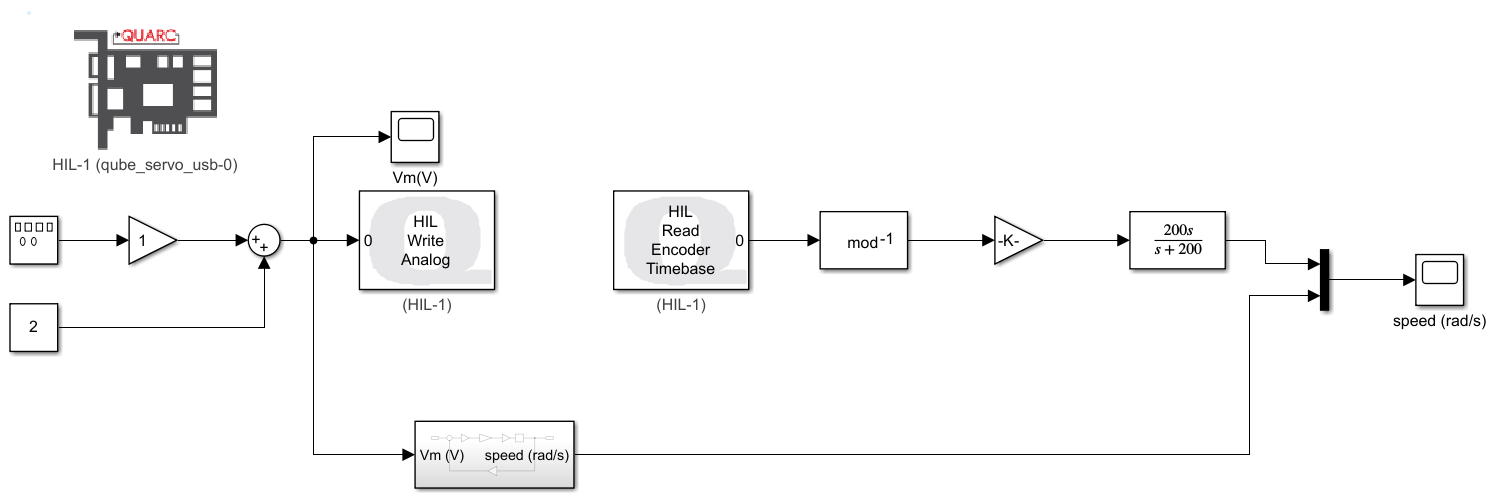
\includegraphics[width=0.75\linewidth]{system.png}
    \caption{Simulink model constructed for analysis}
    \label{fig:1}
\end{figure}
\begin{figure} [H]
    \centering
    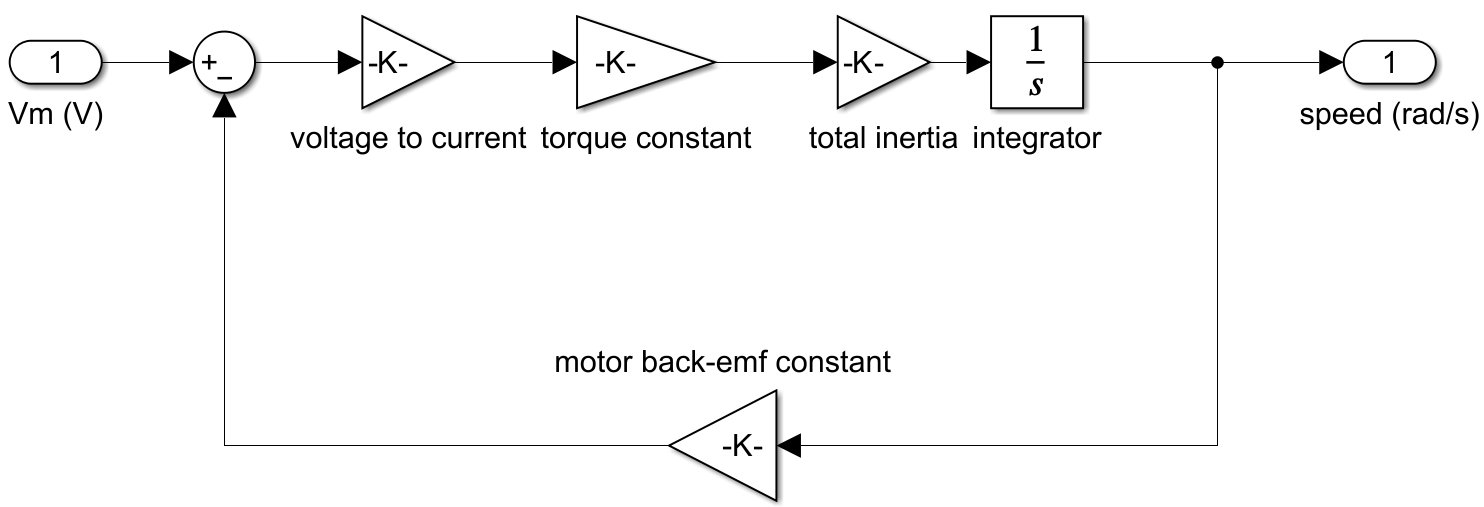
\includegraphics[width=0.75\linewidth]{subsystem.png}
    \caption{Subsystem contained within block}
    \label{fig:2}
\end{figure}

\section{In-Lab exercises and Results}
\subsection{Calculating equivalent moment of inertia}
In order to calculate the equivalent moment of inertia that is acting on the motor shaft, we must consider
\begin{equation}
    J=\frac{1}{2}mr^2,
\end{equation}
and our given values for the masses and radii of the disk, hub, and rotor. We then calculate that $J_\text{disk}=1.6606\times10^{-5} \text{ kg m}^2$, $J_\text{hub}=5.359\times10^{-7} \text{ kg m}^2$, and $J_\text{rotor}=4.0\times10^{-6} \text{ kg m}^2$. Considering
\begin{equation}
    J_\text{eq}=J_\text{disk}+J_\text{hub}+J_\text{rotor},
\end{equation}
we find $J_\text{eq}=2.1142\times10^{-5}\text{ kg m}^2$ for our equivalent moment of inertia that is acting on the motor shaft.

\subsection{QUBE servo model subsystem}
In Figure 2, we observe our model subsystem. We were able to derive this model given the applied torque from the DC motor,
\begin{equation}
    \tau_m=k_mi_m(t),
\end{equation}
the motor shaft equation
\begin{equation}
    J_\text{eq}\dot\omega_m(t)=\tau_m(t),
\end{equation}
and the motor current
\begin{equation}
    i_m(t)=\frac{v_m(t)-k_m\omega_m(t)}{R_m}.
\end{equation}
Substituting, we observe
\begin{equation}
    \dot\omega_m(t)=k_m \left( \frac{v_m(t)-k_m\omega_m(t)}{R_m} \right)\left(\frac{1}{J_\text{eq}}\right),
\end{equation}
which is equivalent to
\begin{equation}
    \omega_m(t)=k_m\int \left( \frac{v_m(t)-k_m\omega_m(t)}{R_m} \right)\left(\frac{1}{J_\text{eq}}\right)\,\mathrm{d}t.
\end{equation}
Creating the block diagram for this equation results us with Figure 1, where $v_m(t)$ is the voltage input, $k_m=0.036\frac{\text{V}}{(\frac{\text{rad}}{\text{s}})}$, $R_m=6.3\Omega$, $\omega_m(t)$ is the speed of the motor shaft, and $J_\text{eq}$ is our previously calculated equivalent moment of inertia.

\subsection{Verifying our system design}
\begin{figure}[H]
    \centering
    \begin{subfigure}[b]{0.45\linewidth}
        \centering
        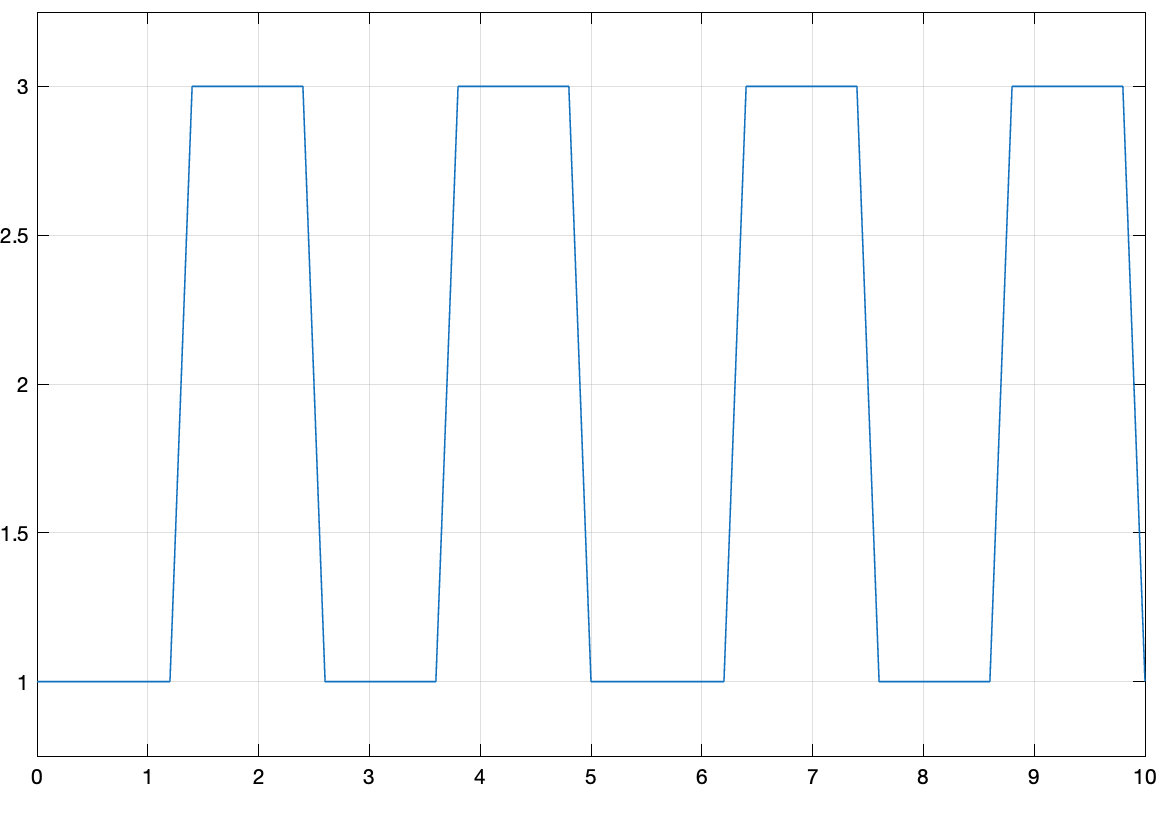
\includegraphics[width=\linewidth]{voltage.png}
        \caption{Voltage input}
        \label{fig:voltage}
    \end{subfigure}
    \hfill
    \begin{subfigure}[b]{0.45\linewidth}
        \centering
        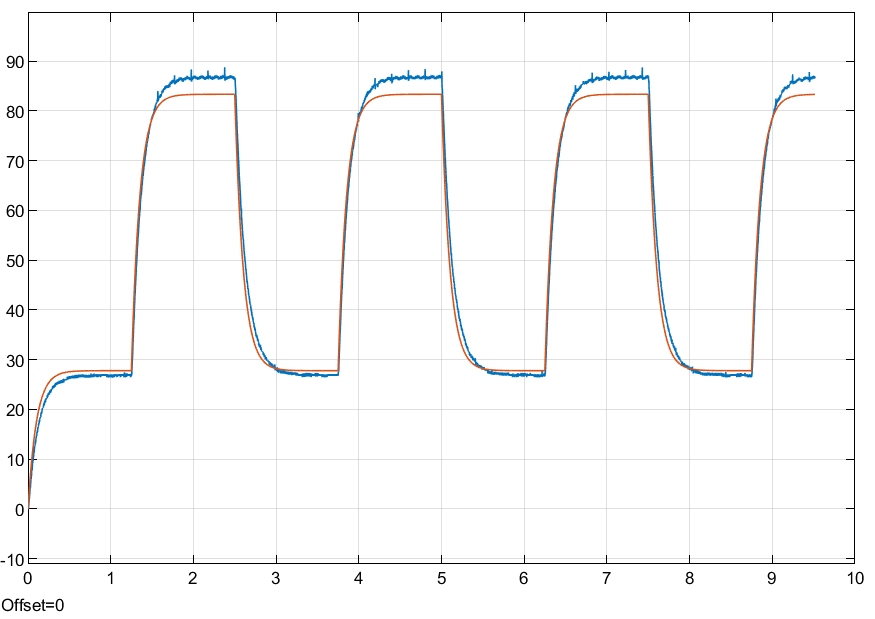
\includegraphics[width=\linewidth]{speed.png}
        \caption{Load speed}
        \label{fig:loadspeed}
    \end{subfigure}
    \caption{System response}
    \label{fig:response}
\end{figure}
Note here that the plot for voltage input is slightly incorrect due to MATLAB's estimation for the plot. The input for the model is a 1-3V 0.4 Hz square wave. In the load speed plot, we observe that our subsystem is an accurate representation of the speed measured by the encoder, considering the error in the encoder measurement. Our plotted representation of the system closely follows the measured load speed line, which verifies our design and calculated values. 

\section{Analysis}
We encountered a variety of issues when working through this lab. One of the main issues that we encountered was inaccuracy in our final plot to verify our subsystem and values. When plotted with the encoder's measurements of the speed, we see a slight inconsistency in the maximum value of the measured speed. Eventually, we were able to determine this resulted from experimental error with our encoder, rather than our calculated values, which we verified to be correct. Aside from this, once we calculated and substituted to obtain equation 7, constructing the subsystem was fairly straightforward. 

\section{Conclusion}
In this lab, we accurately modeled our QUBE-Servo system by using values for the various masses and sizes that are involved in the movement of the servo, and substituted them into a block diagram representation of the system. Through doing so, we were able to create a subsystem that is a near-perfect representation of our original system, as seen in Figures 2 and 3b.

\end{document}